%!TEX builder = latexmk
%!TEX program = xelatex
\documentclass{article}
\usepackage{amsmath,amsfonts,amsthm,amssymb}
\usepackage{setspace}
\usepackage{fancyhdr}
\usepackage{lastpage}
\usepackage{extramarks}
\usepackage{chngpage}
\usepackage{soul,color}
\usepackage{graphicx,float,wrapfig}
\usepackage{CJK}
\usepackage{algorithm}  
\usepackage{algpseudocode} 
\usepackage{enumerate}
\usepackage{longtable}
\usepackage{listings}
\usepackage{framed}
\usepackage{extarrows}
\usepackage{subfigure}
\usepackage{bbm}
\usepackage{hyperref}
\newcommand{\Class}{Fundamentals of Cryptography}
\newcommand{\ClassInstructor}{Wenfei Wu}

% Homework Specific Information. Change it to your own
\newcommand{\Title}{Project Report}
\newcommand{\DueDate}{Jan 15, 2021}
\newcommand{\StudentName}{Runlong Zhou}
\newcommand{\StudentClass}{YaoClass 82}
\newcommand{\StudentNumber}{2018011309}

% In case you need to adjust margins:
\topmargin=-0.45in      %
\evensidemargin=0in     %
\oddsidemargin=0in      %
\textwidth=6.5in        %
\textheight=9.0in       %
\headsep=0.25in         %

% Setup the header and footer
\pagestyle{fancy}                                                       %
\lhead{\StudentName}                                                 %
\chead{\Title}  %
\rhead{\firstxmark}                                                     %
\lfoot{\lastxmark}                                                      %
\cfoot{}                                                                %
\rfoot{Page\ \thepage\ of\ \protect\pageref{LastPage}}                          %
\renewcommand\headrulewidth{0.4pt}                                      %
\renewcommand\footrulewidth{0.4pt}                                      %

%%%%%%%%%%%%%%%%%%%%%%%%%%%%%%%%%%%%%%%%%%%%%%%%%%%%%%%%%%%%%
% Some tools
\newcommand{\enterProblemHeader}[1]{\nobreak\extramarks{#1}{#1 continued on next page\ldots}\nobreak%
                                    \nobreak\extramarks{#1 (continued)}{#1 continued on next page\ldots}\nobreak}%
\newcommand{\exitProblemHeader}[1]{\nobreak\extramarks{#1 (continued)}{#1 continued on next page\ldots}\nobreak%
                                   \nobreak\extramarks{#1}{}\nobreak}%

\newcommand{\homeworkProblemName}{}%
\newcounter{homeworkProblemCounter}%
\newenvironment{homeworkProblem}[1][Problem \arabic{homeworkProblemCounter}]%
  {\stepcounter{homeworkProblemCounter}%
   \renewcommand{\homeworkProblemName}{#1}%
   \section*{\homeworkProblemName}%
   \enterProblemHeader{\homeworkProblemName}}%
  {\exitProblemHeader{\homeworkProblemName}}%

\newcommand{\homeworkSectionName}{}%
\newlength{\homeworkSectionLabelLength}{}%
\newenvironment{homeworkSection}[1]%
  {% We put this space here to make sure we're not connected to the above.

   \renewcommand{\homeworkSectionName}{#1}%
   \settowidth{\homeworkSectionLabelLength}{\homeworkSectionName}%
   \addtolength{\homeworkSectionLabelLength}{0.25in}%
   \changetext{}{-\homeworkSectionLabelLength}{}{}{}%
   \subsection*{\homeworkSectionName}%
   \enterProblemHeader{\homeworkProblemName\ [\homeworkSectionName]}}%
  {\enterProblemHeader{\homeworkProblemName}%

   % We put the blank space above in order to make sure this margin
   % change doesn't happen too soon.
   \changetext{}{+\homeworkSectionLabelLength}{}{}{}}%

\newcommand{\Answer}{\textbf{Answer:} }
\newcommand{\Acknowledgement}[1]{\ \\{\bf Acknowledgement:} #1}

%%%%%%%%%%%%%%%%%%%%%%%%%%%%%%%%%%%%%%%%%%%%%%%%%%%%%%%%%%%%%


%%%%%%%%%%%%%%%%%%%%%%%%%%%%%%%%%%%%%%%%%%%%%%%%%%%%%%%%%%%%%
% Make title
\title{\textmd{\bf \Class: \Title}\\{\large Instructed by \textit{\ClassInstructor}}\\\normalsize\vspace{0.1in}\small{Due\ on\ \DueDate}}
\date{}
\author{\textbf{\StudentName}\ \ \StudentClass\ \ \StudentNumber}
%%%%%%%%%%%%%%%%%%%%%%%%%%%%%%%%%%%%%%%%%%%%%%%%%%%%%%%%%%%%%

\definecolor{shadecolor}{rgb}{0.92,0.92,0.92}

%%%%%%%%%%%%%%%%%%%%%%%%%%%%%%%%%%%%%%%%%%%%%%%%%%%%%%%%%%%%%
% Listing Settings
\definecolor{mygreen}{rgb}{0,0.6,0}
\definecolor{mygray}{rgb}{0.5,0.5,0.5}
\definecolor{mymauve}{rgb}{0.58,0,0.82}

\lstset{
  aboveskip=1em,                   % above skip space
  backgroundcolor=\color[rgb]{0.9,0.9,0.9},
                                   % choose the background color; you must add \usepackage{color} or \usepackage{xcolor}; should come as last argument
  basicstyle=\ttfamily,            % the size of the fonts that are used for the code
  breakatwhitespace=false,         % sets if automatic breaks should only happen at whitespace
  breaklines=true,                 % sets automatic line breaking
  captionpos=b,                    % sets the caption-position to bottom
  commentstyle=\color{mygreen},    % comment style
  deletekeywords={...},            % if you want to delete keywords from the given language
  escapeinside={\%*}{*)},          % if you want to add LaTeX within your code
  extendedchars=true,              % lets you use non-ASCII characters; for 8-bits encodings only, does not work with UTF-8
  frame=single,	                   % adds a frame around the code
  keepspaces=true,                 % keeps spaces in text, useful for keeping indentation of code (possibly needs columns=flexible)
  keywordstyle=\color{blue},       % keyword style
  morekeywords={algexpr, frac, sqrt, pwr, b1, b2, b3, ln, sin, term},  
                                   % if you want to add more keywords to the set
  numbers=left,                    % where to put the line-numbers; possible values are (none, left, right)
  numbersep=5pt,                   % how far the line-numbers are from the code
  numberstyle=\color{mygray},      % the style that is used for the line-numbers
  rulecolor=\color{black},         % if not set, the frame-color may be changed on line-breaks within not-black text (e.g. comments (green here))
  showspaces=false,                % show spaces everywhere adding particular underscores; it overrides 'showstringspaces'
  showstringspaces=false,          % underline spaces within strings only
  showtabs=false,                  % show tabs within strings adding particular underscores
  stepnumber=5,                    % the step between two line-numbers. If it's 1, each line will be numbered
  stringstyle=\color{mymauve},     % string literal style
  tabsize=2,	                   % sets default tabsize to 2 spaces
  title=\lstname,                  % show the filename of files included with \lstinputlisting; also try caption instead of title
  xleftmargin=2em,                 % left margin
  xrightmargin=2em,                % right margin
}
%%%%%%%%%%%%%%%%%%%%%%%%%%%%%%%%%%%%%%%%%%%%%%%%%%%%%%%%%%%%%


\renewcommand{\algorithmicrequire}{\textbf{Input:}}  % Use Input in the format of Algorithm  
\renewcommand{\algorithmicensure}{\textbf{Output:}} % Use Output in the format of Algorithm  


\newcommand*{\dif}{\mathop{}\!\mathrm{d}}
\newcommand*{\img}{\mathrm{i}}
\newcommand*{\dps}{\displaystyle}
\newcommand*{\lf}{\left\lfloor}
\newcommand*{\rf}{\right\rfloor}
\newcommand*{\lc}{\left\lceil}
\newcommand*{\rc}{\right\rceil}
\newcommand*{\ovt}[2]{\dps{\mathop{#1}^{#2}}}

\newtheorem{lma}{Lemma}

\newcommand{\lm}[1]{\textbf{Lemma \ref{#1}}}
\newcommand{\lgd}[2]{\left(\frac{#1}{#2}\right)}
\newcommand{\ds}[2]{\dps \frac{\partial #1}{\partial #2}}
\newcommand{\bds}[2]{\dps \frac{\partial}{\partial #2}\left(#1\right)}
\newcommand{\Eds}[2]{\dps \frac{\partial^2 #1}{\partial #2^2}}
\newcommand{\eds}[3]{\dps \frac{\partial^2 #1}{\partial #2\partial #3}}
\newcommand{\E}[1]{\mathbb{E}\left[#1\right]}
\newcommand{\Var}[1]{\mathrm{Var}\left[#1\right]}
\newcommand{\Cov}[1]{\mathrm{Cov}\left[#1\right]}

\newcommand{\Fig}[1]{\textbf{Figure \ref{#1}}}

\begin{document}
\begin{spacing}{1.1}
\maketitle \thispagestyle{empty}
%\cite{}
%%%%%%%%%%%%%%%%%%%%%%%%%%%%%%%%%%%%%%%%%%%%%%%%%%%%%%%%%%%%%
% Begin edit from here

\section{Experiment Setup}

\begin{enumerate}

\item The framework is an MPC framework called
\href{https://github.com/samee/obliv-c}{Obliv-C}. I used the code contained in
\href{https://github.com/mpc-sok/frameworks}{MPC-SoK}.

\item I provided two experiments, inner product and cross tabs. Before building the
framework, we should first generate corresponding test data. Enter \texttt{non-crypto}
folder and choose the experiments you want, then execute
\begin{shaded}
\texttt{make gendata\\
./gendata}
\end{shaded}
Finally, copy the two input files \texttt{input*.txt} into
\texttt{sok\_obliv-c/source/<experiment>}.

\item The main prerequisite is \texttt{docker.io}. To build and run the framework, enter 
\texttt{sok\_obliv-c} folder and execute
\begin{shaded}
\texttt{docker build -t obliv-c .}
\end{shaded}
then execute
\begin{shaded}
\texttt{docker run -it --rm obliv-c}
\end{shaded}

\item 
Then, enter either \texttt{innerProd} or \texttt{crossTabs}, execute
\begin{shaded}
\texttt{make\\
time ./a.out 1234 -- input1.txt \& ./a.out 1234 localhost input2.txt}
\end{shaded}
The result and executing time will be printed on console.

\end{enumerate}


\section{Framework Capabilities}

This framework is C-style compatible.

\begin{enumerate}

\item Operators: addition, multiplication, bit-wise operations, etc.

\item Data type: bool, char, int, short, long, long long, float

\item Control flow: loop, if-else and any common C control flow

\item Function: supported

\item Global/local variable: the framework itself is an embedded function, so
global vairables are not supported, but local variables are supported.

\end{enumerate}


\section{Performance}

\subsection{Inner product}

\begin{enumerate}

\item \textbf{Description:} It computes inner product of two $n$-dimension integer vectors.
Two parties each hold one vector.

\item \textbf{Result:}

\begin{figure}[H] 
\centering 
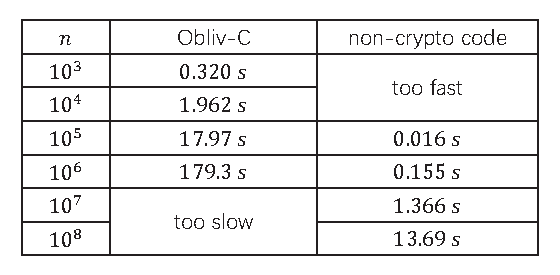
\includegraphics[scale=1]{dot.eps}
\caption{Execution time when $n$ varies}
\label{dot}
\end{figure}

From \Fig{dot}, Obliv-C implements a protocol with time complexity linear in $n$. However,
the time to setup channel takes majority when $n$ is small, so the overall time seemes not
linear in $n$. The performance of Obliv-C is around $100$ times slower than simple, 
non-crypto code.

\end{enumerate}

\subsection{Cross tabs}

\begin{enumerate}

\item \textbf{Description:} Party A holds a list containing (ID, category) pairs, while
party B holds a list containing (ID, data) pairs. They want to compute a list of
(category, sum of data in this category) pairs.

\item \textbf{Result:}

\begin{figure}[H] 
\centering 
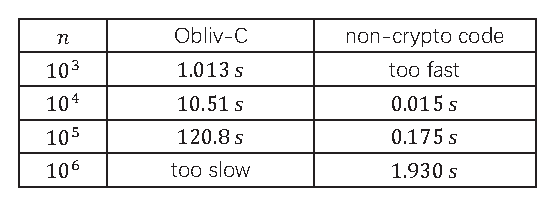
\includegraphics[scale=1]{cross.eps}
\caption{Execution time when $n$ varies}
\label{cross}
\end{figure}

From \Fig{cross}, Obliv-C implements a protocol with time complexity almost linear in $n$.
In fact, it implements a sort inside, so the real time complexity is $O(n\log n)$,
and the non-crypto code uses three \texttt{std::map}s.
This experiment shows a separation of $1000$ times.

\end{enumerate}

% End edit to here
%%%%%%%%%%%%%%%%%%%%%%%%%%%%%%%%%%%%%%%%%%%%%%%%%%%%%%%%%%%%%

\end{spacing}
\end{document}

%%%%%%%%%%%%%%%%%%%%%%%%%%%%%%%%%%%%%%%%%%%%%%%%%%%%%%%%%%%%%
